\subsection{航点控制逻辑1}
在引入算法之前,我们需要先了解一个概念"半平面(half-plane)",
半平面是被用来指定是否航点切换的核心条件,
通过无人机当前位置和半平面的几何关系,来判定航点是到达。具体的几何关系式如下:
    \begin{equation} % 等式
        \begin{aligned}
            \textit{H}(r,n) = \left\{ p \in R^{3} : \left(p-r\right)^{T}n \geq 0 \right\} 
        \end{aligned}
    \end{equation}
    \par 其中的 $r$ 为正在执行的目标航点,$n$为该半平面的法向量,$p$为无人机的当前位置,物理模型如图\ref{half_plane}所示。定义了一个单位向量$q_{i}$和 $n_{i}$,
    $q_{i}$ 是航线 $\overline{w_{i}w_{i+1}}$ 的单位方向向量,所以存在一个三维向量$n_{i}$,可以把航线 $\overline{w_{i-1}w_{i}}$ 和 $\overline{w_{i}w_{i+1}}$ 分隔开.
    \begin{equation}
        \begin{cases}
        &q_{i} \triangleq \frac{w_{i+1}-w_{i}}{\lVert w_{i+1}-w_{i} \rVert} \\
        &n_{i} \triangleq \frac{q_{i-1}+q_{i}}{\lVert q_{i-1}+q_{i} \rVert}
        \end{cases}
    \end{equation}
    \begin{figure}[b]
        \centering
        \subfigure[]{
            \begin{minipage}[t]{0.48\linewidth}
                \centering
                    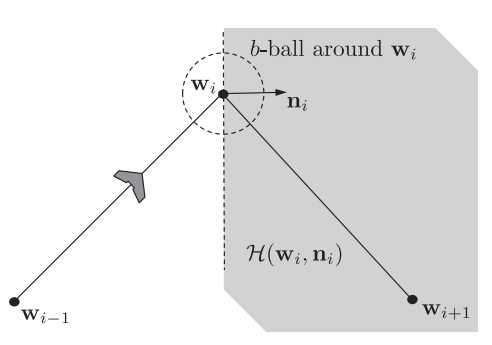
\includegraphics[width=0.7\textwidth]{pictures/half_plane.png}
                \label{half_plane}
            \end{minipage}
        }
        \subfigure[]{
            \begin{minipage}[t]{0.48\linewidth}
                \centering
                    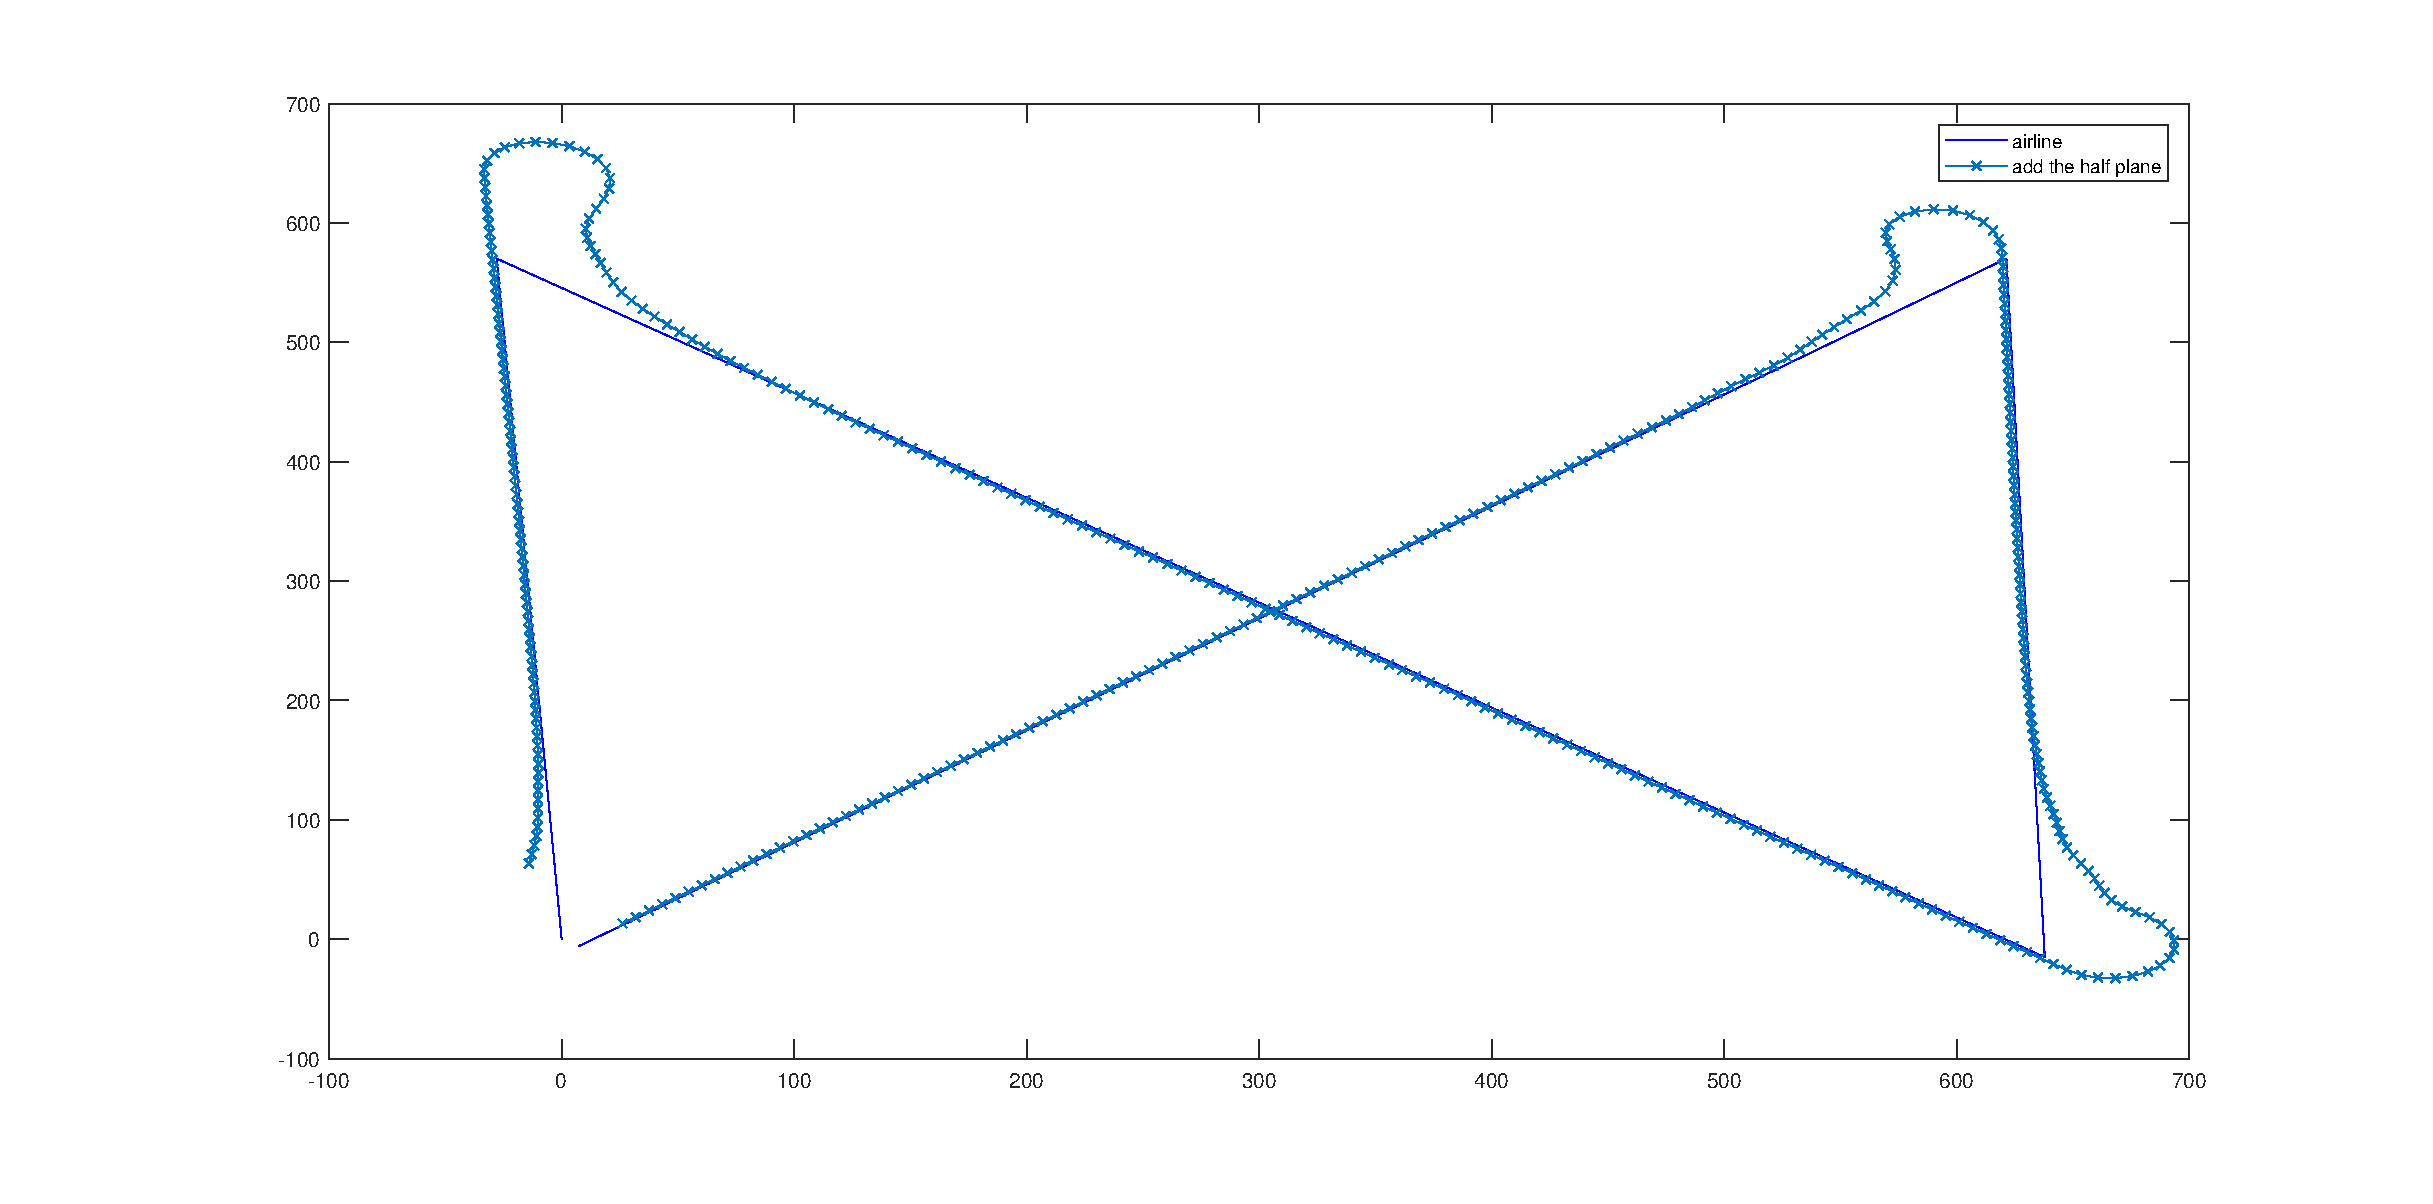
\includegraphics[width=\textwidth]{pictures/eps/algorithm5.eps}
                \label{straight_}
            \end{minipage}
        }
        \caption{straight line}
    \end{figure}
    \begin{figure}[h]
        \centering
        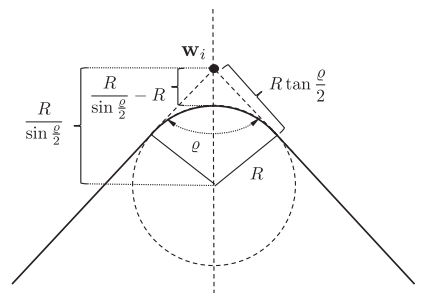
\includegraphics[width=0.5\textwidth]{pictures/algo6_2.png}
        \caption{插入fillet}
        \label{figure:alg6}
    \end{figure}
    \par 无人机从航点$w_{i-1}$到$w_{i}$的飞行过程中,若到达两条航线所生成的半平面,则认为到达了目标航点,
    航线进行切换。飞行控制逻辑包含直线飞行控制和盘旋飞行控制,在直线飞行的过程中,
    航点切换依附着算法\ref{algo5:ref}(航点控制逻辑1)。
    
    第一次执行该算法时候,需要初始化i的值,让其等于2,见\ref{algo5:ref:init};UAV会执行航线$\overline{w_{i-1}w_{i}}$,在算法第4、5行分别定义针对当前执行航点的$r$和$q$,第6行定义了下一条航线的单位方向向量,第7行是航线 $\overline{w_{i-1}w_{i}}$ 和 $\overline{w_{i}w_{i+1}}$ 所生成半平面的法向量,8行到10行进行位置判定,若满足某个关系式,即若无人机穿过半平面,
    那么就要切换航点,执行下一条航线,直到最后一个航点序列号减一。
    \begin{algorithm}[h]
            \caption{Follow Waypoints:(r, q)=followWpp($\textit{W}$, p)}
            \label{algo5:ref}
            \begin{algorithmic}[1]
                \ENSURE Waypoints path $\textit{W}$ = $\left\{ w_{1}, \dots, w_{N} \right\}$, MAV position p=$(p_{n}, p_{e}, p_{d})^{T}$.
                \REQUIRE N $\geq$ 3
                \IF {New waypoints path $\textit{W}$ is received}
                    \STATE Initialize waypoint index: $i$ $\gets$ 2
                    \label{algo5:ref:init}
                \ENDIF
                \STATE $r$ $\gets$ $w_{i-1}$

                \STATE $q_{i-1}$ $\gets$ $\frac{w_{i}-w_{i-1}}{\lVert w_{i}-w_{i-1} \rVert}$
                \STATE $q_{i}$ $\gets$ $\frac{w_{i+1}-w_{i}}{\lVert w_{i+1}-w_{i} \rVert}$
                \STATE $n_{i}$ $\gets$ $\frac{q_{i-1}+q_{i}}{\lVert \| q_{i-1}+q_{i} \rVert}$
                \IF {$p$ $\in$ $\textit{H}(w_{i},n_{i})$}
                    \STATE Increment $i$ $\gets$ $\left(i+1\right)$ until $i$ = $N$ - 1
                \ENDIF
                \RETURN $r$, $q$=$q_{i-1}$ at each time step.  % this command shows "Output"
            \end{algorithmic}
        \end{algorithm}

        \par 算法\ref{algo5:ref}产生的飞行效果如图\ref{straight_}所示,
        很明显,但在直线飞行航点之间切换的时候,因忽略转弯时无人机初始动量的问题,造成了一段很长的转换缓冲距离,致使飞行效果很差,航线不平滑。
    \subsection{航点控制逻辑2}
        \par 对其优化有两种方法, 一是当无人机当前的位置在当前执行的航线上的投影到该航线的起点的\textcolor{blue}{距离占整个比重的90\%}的时候, 进行航点切换;
    
    另外一个较优的改进方法是为其增加一个\textcolor{blue}{圆角(fillet)},如图\ref{fig:algor6}所示,在航点 $w_{i}$ 附近,生成一个盘旋中心,
 让其使得无人机在执行该航点的时候,以圆弧的方式进入到下一条航线,这么航线飞行出来的效果较好。
 定义航线$\overline{w_{i-1}w_{i}}$ 和$\overline{w_{i}w_{i+1}}$的角度为 $\varrho$:
 \begin{figure}[h]
    \centering
    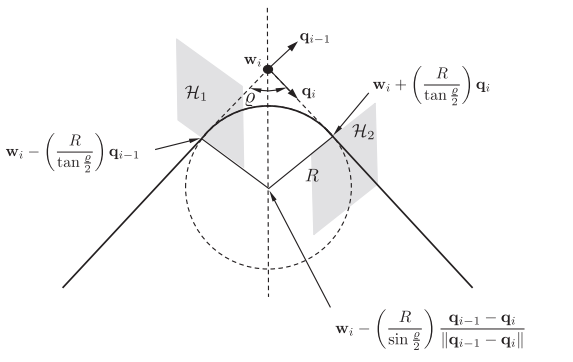
\includegraphics[width=0.6\textwidth]{pictures/algo6_3.png}
    \caption{将半平面和fillet进行结合}
    \label{fig:algor6}
\end{figure}
    \begin{equation}
        \varrho \triangleq cos^{-1}(-q_{i-1}^{T}q_{i})
    \end{equation}
    
    \begin{algorithm}[h]
            \caption{Follow Waypoints with Fillet:(flag, r, q, c, $\rho$, $\lambda$)=followWppFillet($\textit{W}$, p, $R$)}
            \label{algo6:ref}
            \begin{algorithmic}[1]
                \ENSURE Waypoints path $\textit{W}$ = $\left\{ w_{1}, \dots, w_{N} \right\}$, MAV position p=$(p_{n}, p_{e}, p_{d})^{T}$, fillet radius $R$
                \REQUIRE N $\geq$ 3
                \IF {New waypoints path $\textit{W}$ is received}
                    \STATE Initialize waypoint index: $i$ $\gets$ 2, and state machine: state $\gets$ 1
                \ENDIF
                \STATE $q_{i-1}$ $\gets$ $\frac{w_{i}-w_{i-1}}{\lVert w_{i}-w_{i-1} \rVert}$
                \STATE $q_{i}$ $\gets$ $\frac{w_{i+1}-w_{i}}{\lVert w_{i+1}-w_{i} \rVert}$
                \STATE $\varrho$ $\gets$ $cos^{-1}(-q_{i-1}^{T}q_{i})$
                \IF {state = 1}
                    \STATE flag $\gets$ 1
                    \STATE $r$ $\gets$ $w_{i-1}$
                    \STATE $q$ $\gets$ $q_{i-1}$
                    \STATE $z$ $\gets$ $w_{i} - \frac{R}{tan(\frac{\varrho}{2})}q_{i-1}$

                    \IF {$p$ $\in$ $\textit{H}(z,q_{i-1})$}
                        \STATE state $\gets$ 2
                    \ENDIF
                \ELSIF{state = 2}
                    \STATE flag $\gets$ 2
                    \STATE $c$ $\gets$ $w_{i} - \frac{R}{sin(\frac{\varrho}{2})}\frac{q_{i-1}-q_{i}}{\lVert q_{i-1}-q_{i} \rVert}$
                    \STATE $\rho$ $\gets$ $R$
                    \STATE $\lambda$ $\gets$ $sign(q_{i-1,n}q_{i,e}-q_{i-1,e}q_{i,n})$
                    \STATE $z$ $\gets$ $w_{i} + \frac{R}{tan(\frac{\varrho}{2})}q_{i}$
                    \IF {$p$ $\in$ $\textit{H}(z,q_{i})$}
                        \STATE $i$ $\gets$ $\left(i+1\right)$ until $i$ = $N$ - 1
                        \STATE state $\gets$ 1
                    \ENDIF
                \ENDIF
                \RETURN flag, $r$, $q$, $c$, $\rho$,$\lambda$.  % this command shows "Output"
            \end{algorithmic}
        \end{algorithm}
在图\ref{figure:alg6}中,假定fillet的半径为R,那么圆弧和两条航线的切点距航点$w_{i}$的距离为$\frac{R}{tan(\frac{\varrho}{2})}$
    且航点$w_{i}$和fillet的中心的距离是$\frac{R}{sin(\frac{\varrho}{2})}$,所以航点$w_{i}$距圆角fillet的最短距离为$\frac{R}{sin(\frac{\varrho}{2})}$ - $R$.
    为了让其直线控制逻辑和圆弧控制逻辑\upcite{8}更好的结合,对此也引进来了"半平面"。
    在图\ref{fig:algor6}中,
    定义了两个半平面 \textit{$H_{1}$} 和 \textit{$H_{2}$}。飞机在未进入半平面 \textit{$H_{1}$}
    的时候,执行直线控制逻辑;当进入到 \textit{$H_{1}$} 的时候,执行圆弧控制逻辑,此时,圆弧的中心是 $c$,半径是 $\rho$;直到无人机进入 \textit{$H_{2}$} ,切换到直线控制逻辑。
    在算法\ref{algo6:ref}(航点控制逻辑2)中,给出了详细的逻辑梳理。
    圆角的中心 $c$, 第一个半平面、第二半平面与圆角相交的点 $r_{1}$ 和 $r_{2}$ 定义如下:
        \begin{align}
            &c = w_{i} - \frac{R}{sin(\frac{\varrho}{2})} \frac{q_{i-1}-q_{i}}{\lVert q_{i-1}-q_{i} \rVert} \\
            &r_{1} = w_{i} - \left( \frac{R}{tan(\frac{\varrho}{2})} \right)q_{i-1} \\
            &r_{2} = w_{i} + \left( \frac{R}{tan(\frac{\varrho}{2})} \right)q_{i}
        \end{align}
    \par其中的向量 $q_{i-1}$ 和 $q_{i}$ 分别为两条航线的单位方向向量。算法\ref{algo6:ref}中,若一条新的航线被接收,那么航点序列号和state的值也会在第2行进行更新,向量$q_{i-1}$ 和 $q_{i}$,以及$\varrho$在4到6行计算;
    当state = 1的时候,调用直线控制逻辑,执行航线 $\overline{w_{i-1}w_{i}}$,同时计算相对应的 $r$ 和 $q$,在第11到14行判断是否到达第一个半平面;若无人机穿过第一个半平面,朝着第二个半平面飞去的时候,state = 2,执行曲线控制逻辑,对应的圆心为$c$,半径为$\rho$,飞行的方向(逆时针,或顺时针)为$\lambda$;若无人机穿过第二个半平面,则state赋值为1,执行直线控制逻辑。

    
    \subsection{算法优化} 
    算法\ref{algo5:ref}和算法\ref{algo6:ref}执行效果对比如图\ref{algo5_com_6}所示, 图\ref{5_6_bigger}是将右下角转弯轨迹放大之后得到的. 很显然, 从总体路径长度最优的角度来看, 后者的总体路径长度要明显比前者总体路径长度短很多, 执行效率也会优于前者.
    \begin{figure}[h]
        \centering
        \subfigure[]{
            \begin{minipage}[t]{0.48\linewidth}
                \centering
                    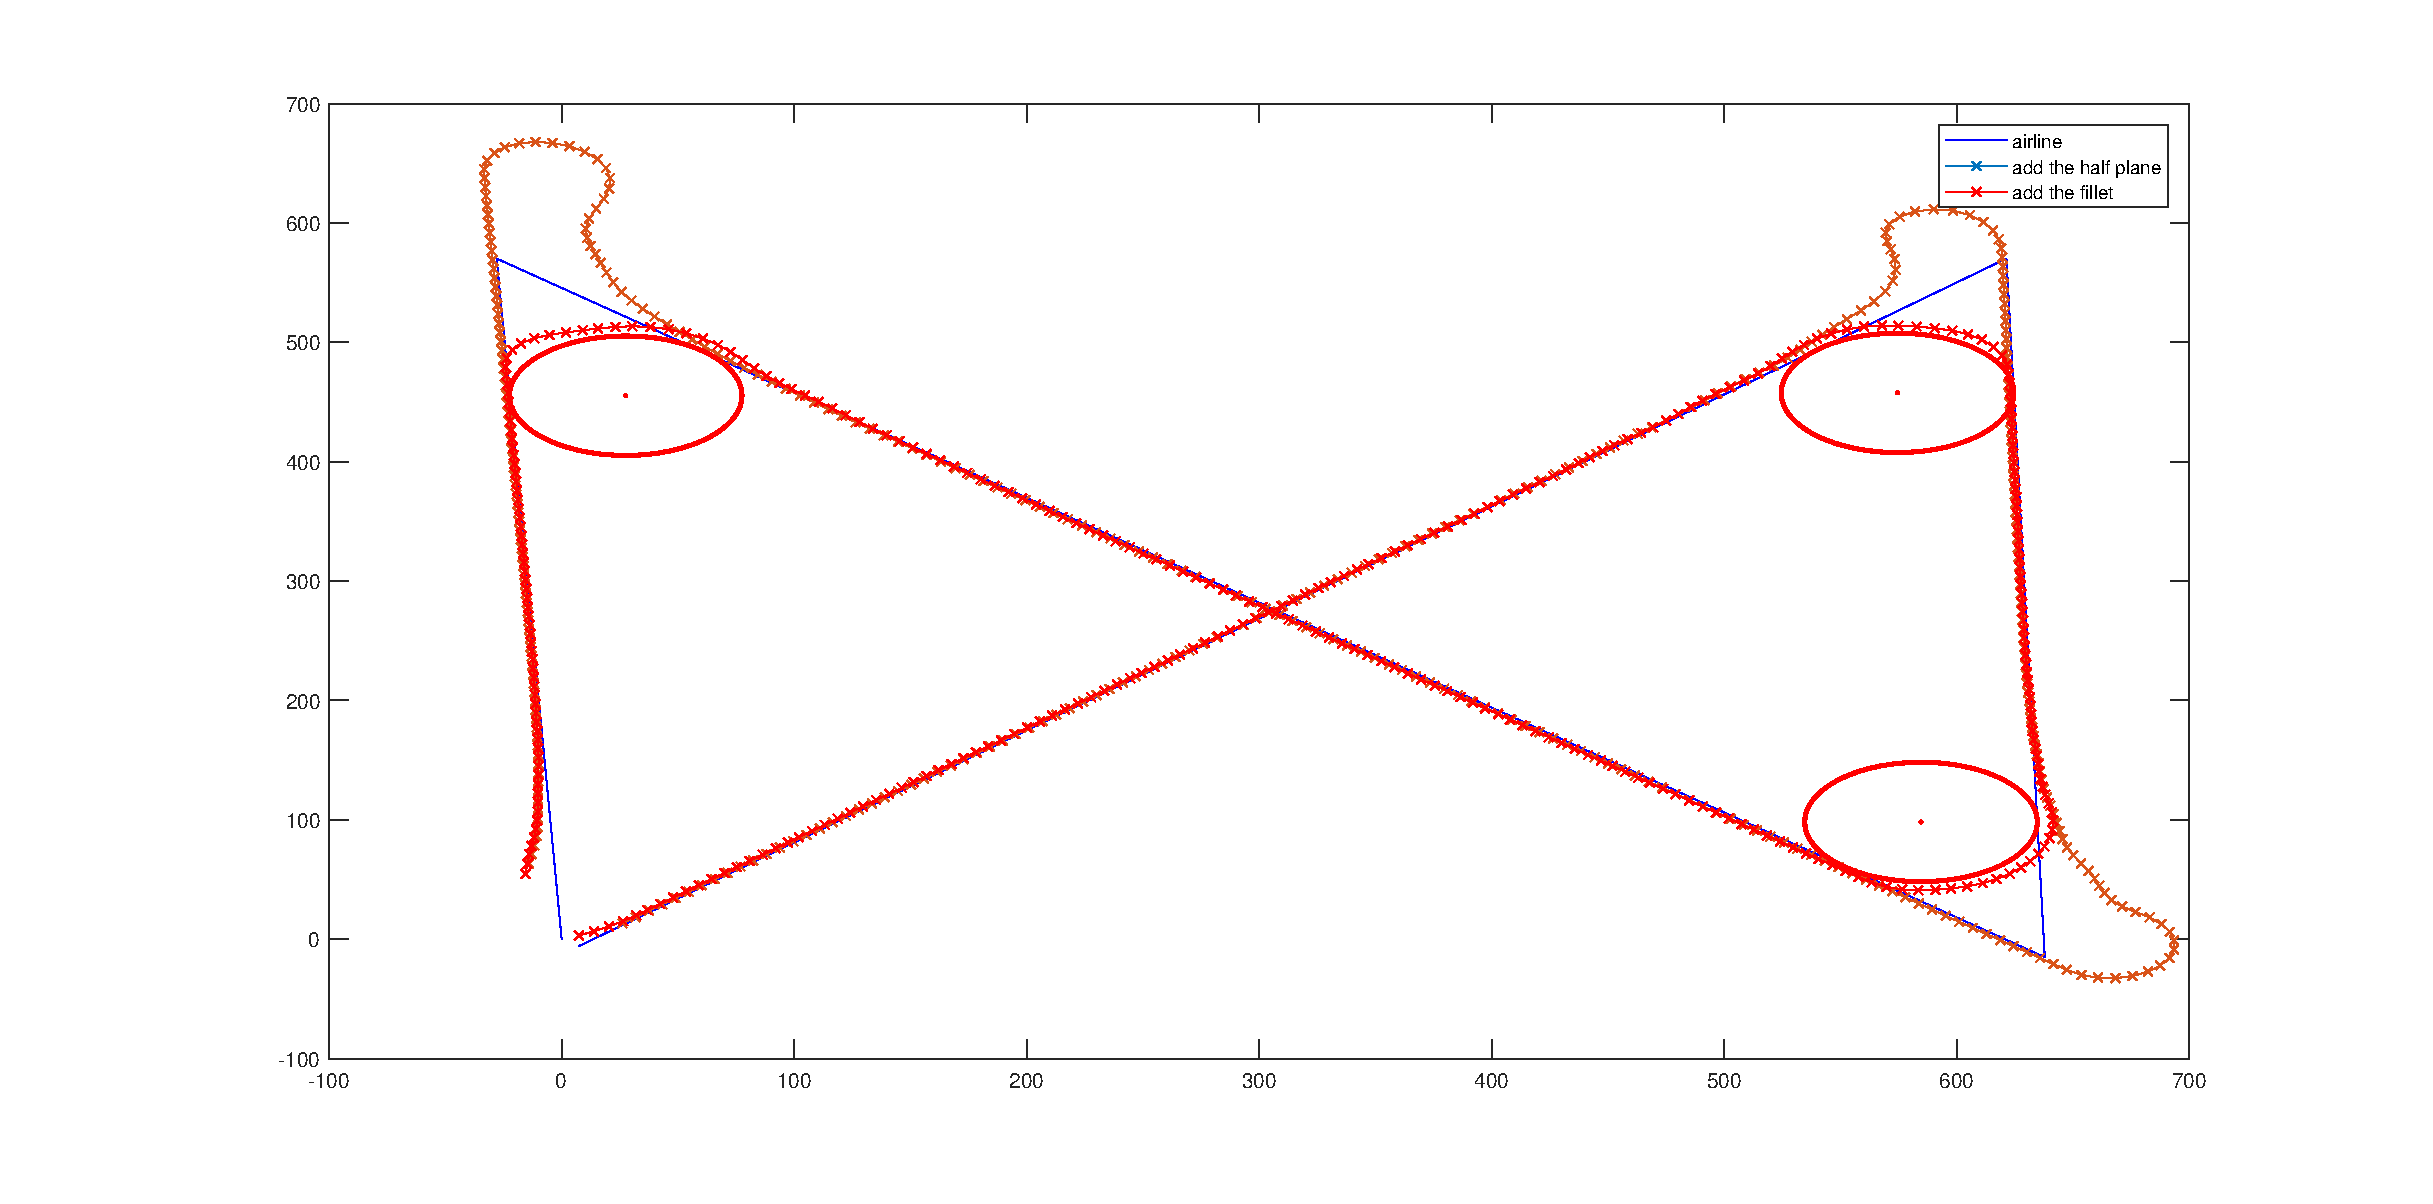
\includegraphics[width=\textwidth]{pictures/eps/algorithm5_6.eps}
                \label{algo5_com_6}
            \end{minipage}
        }
        \subfigure[]{
            \begin{minipage}[t]{0.48\linewidth}
                \centering
                    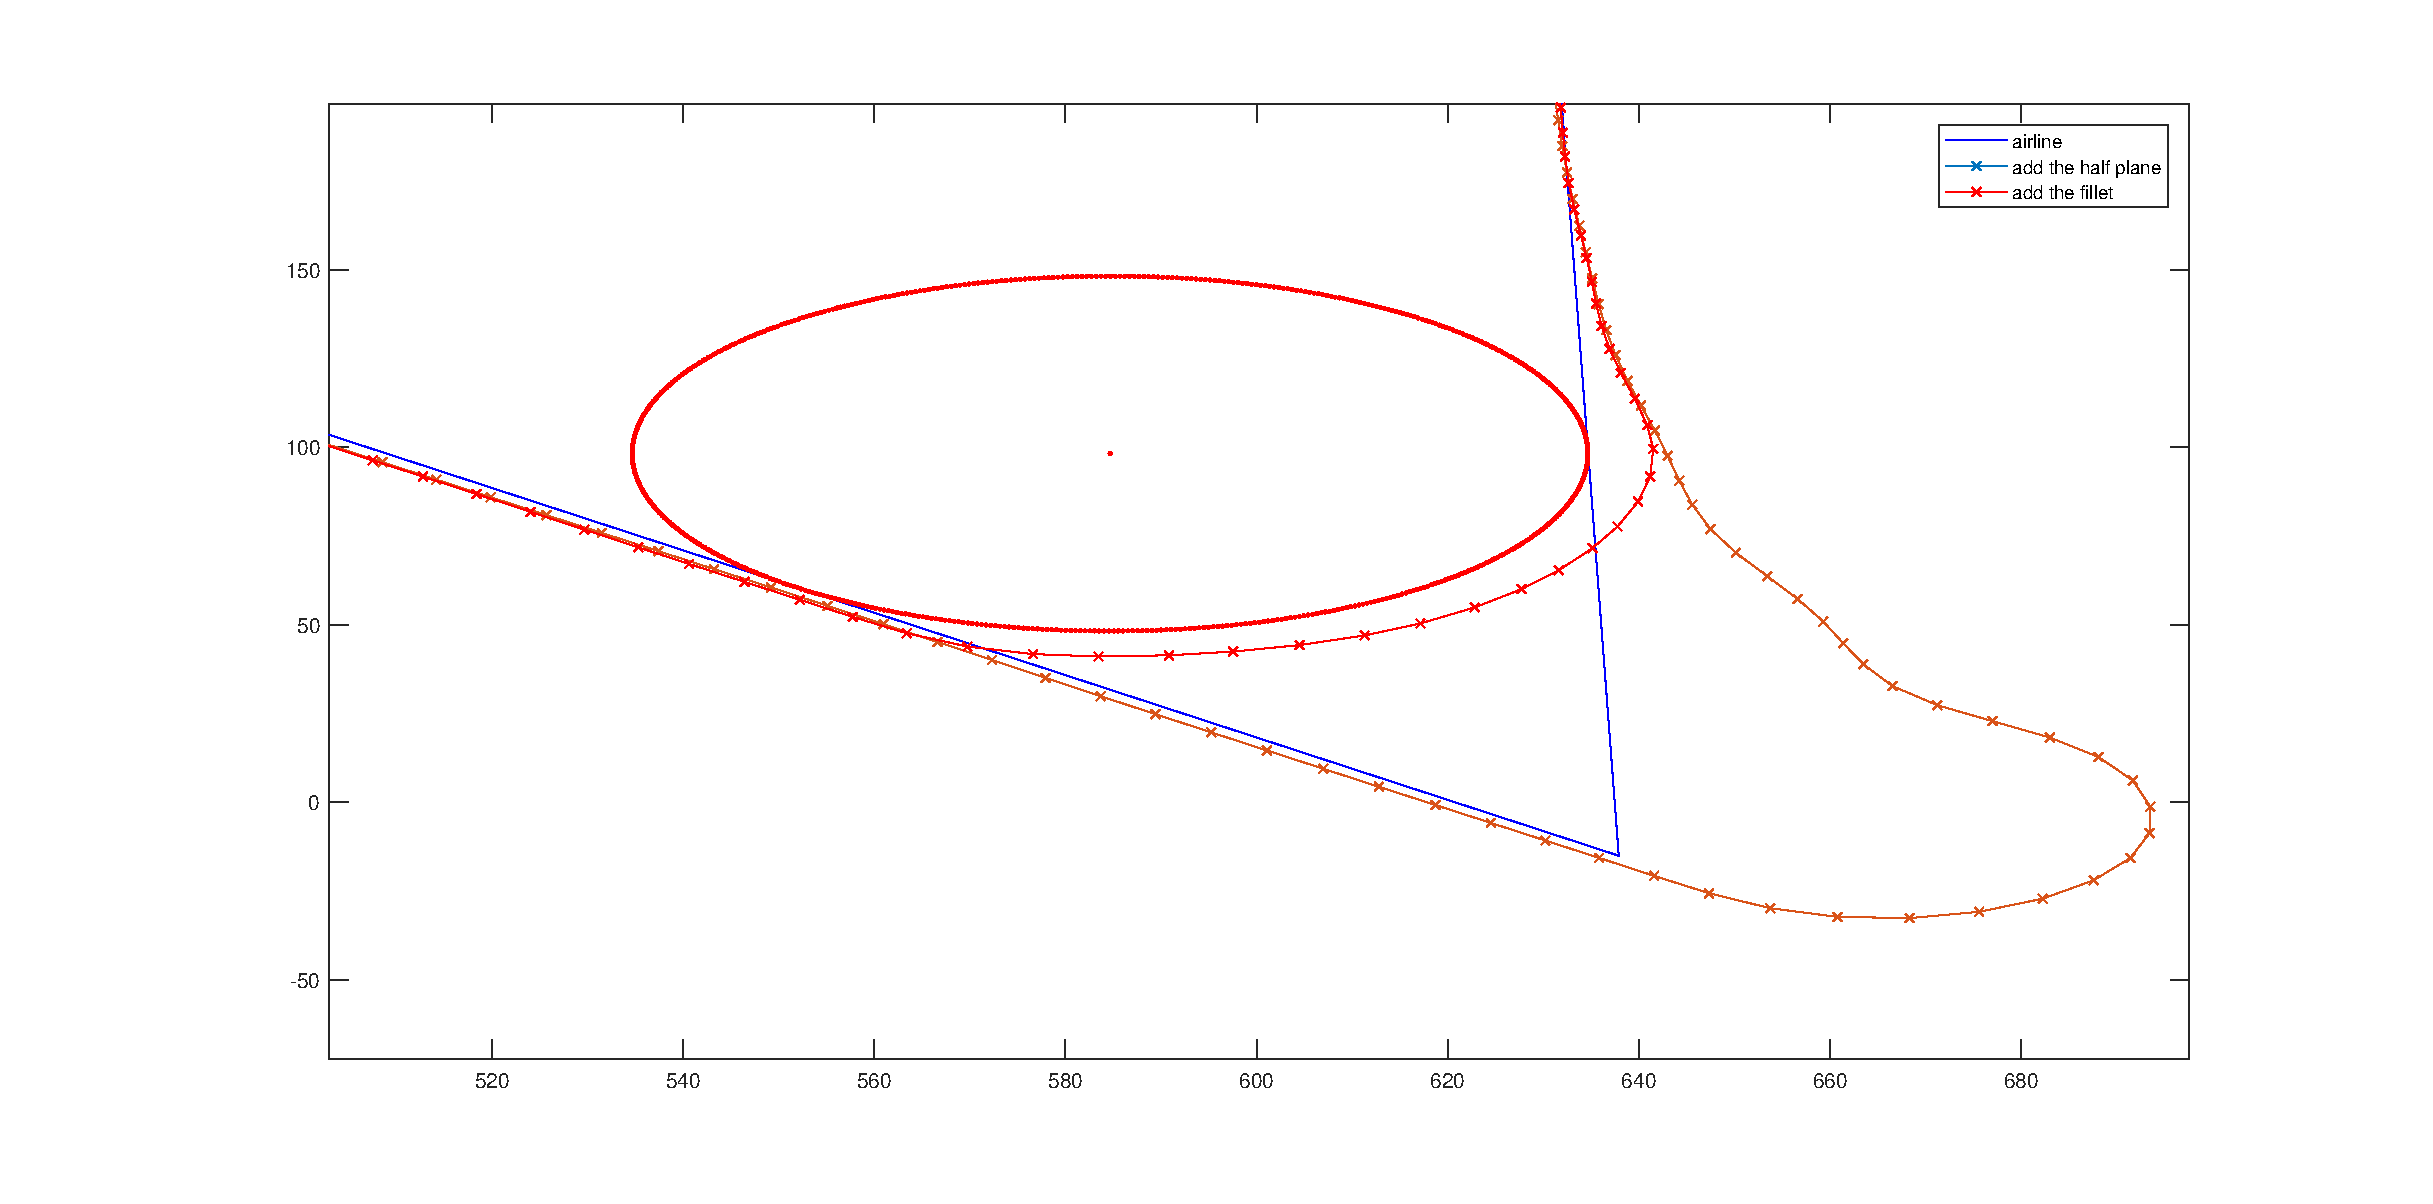
\includegraphics[width=\textwidth]{pictures/eps/algorithm5_6_1.eps}
                \label{5_6_bigger}
            \end{minipage}
        }
        \caption{comparing}
    \end{figure}
    尽管如此, 算法\ref{algo6:ref}在转弯的时候, 对初试惯性动量考虑的不太周到, 存在一些瑕疵, 如图\ref{fig:algo6}所示.
    虽然在算法\ref{algo6:ref}中, 模型建立是以fillet和航线相切的情况来考虑的, 但在仿真平台中, 无人机的并不是以期望空速来飞行, 而是以期望空速(airspeed)和风速(wind speed)叠加之后形成的地速(ground speed)来飞行. 由于风速大小的不确定性, 造成了飞行效果差强人意.
    \begin{figure}[htbp]
        \centering
        \subfigure[]{
            \begin{minipage}[t]{0.48\linewidth}
                \centering
                    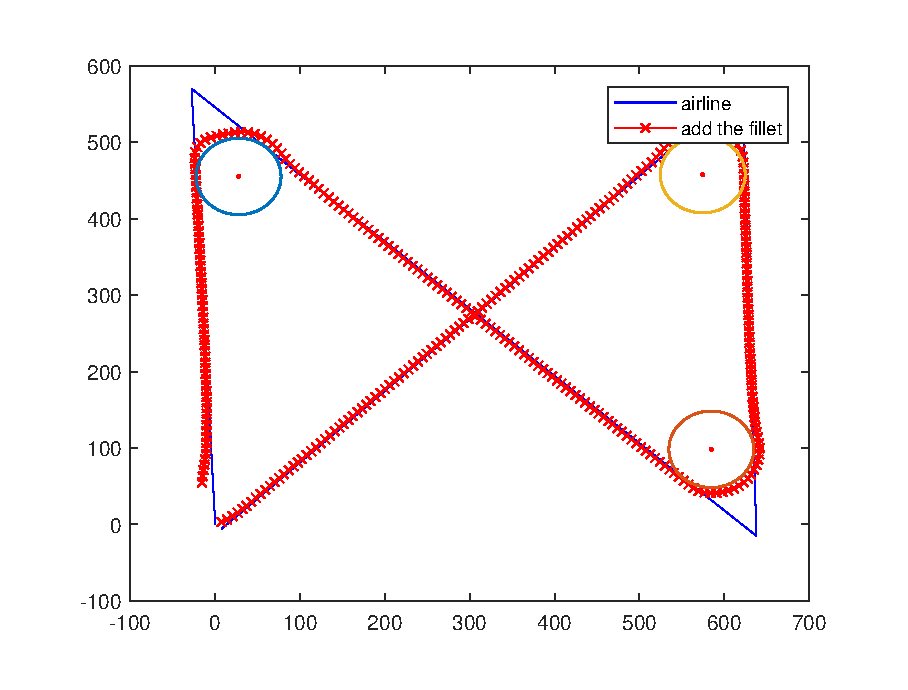
\includegraphics[width=0.8\textwidth]{pictures/eps/algorithm6.eps}
                \label{fig:algo6}
            \end{minipage}
        }
        \subfigure[]{
            \begin{minipage}[t]{0.48\linewidth}
                \centering
                    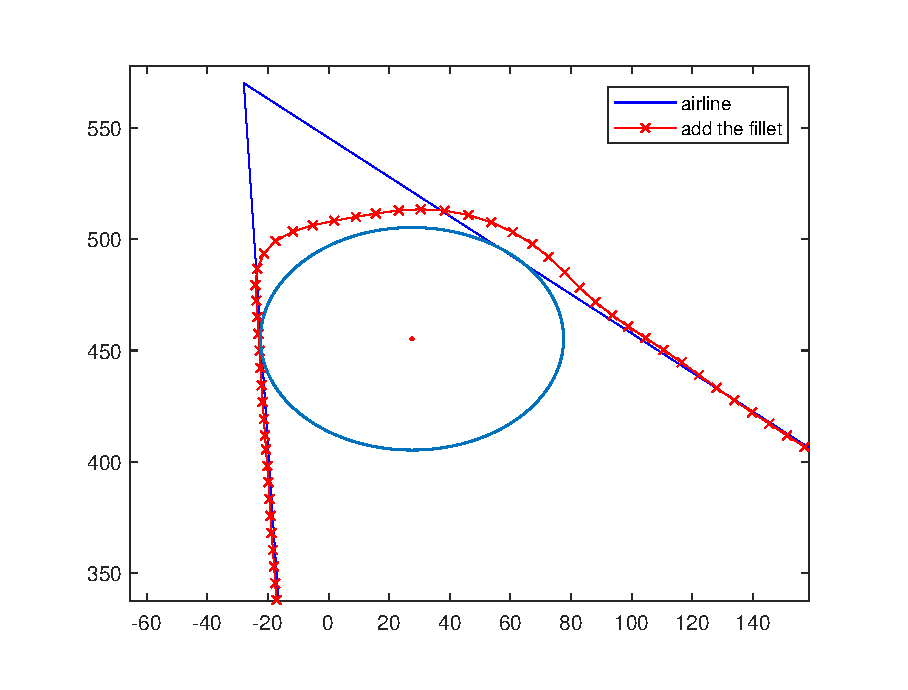
\includegraphics[width=0.8\textwidth]{pictures/eps/algorithm6_1.eps}
                \label{fig:algo6_1}
            \end{minipage}
        }
        \\
        \subfigure[]{
            \begin{minipage}[t]{0.48\linewidth}
                \centering
                    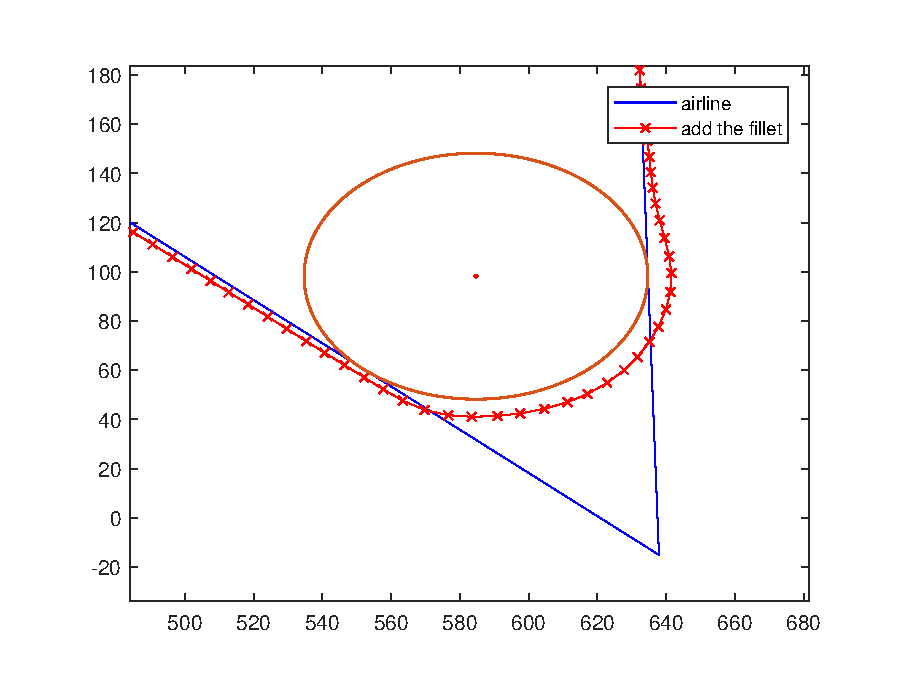
\includegraphics[width=0.8\textwidth]{pictures/eps/algorithm6_2.eps}
                \label{fig:algo6_2}
            \end{minipage}
        }
        \subfigure[]{
            \begin{minipage}[t]{0.48\linewidth}
                \centering
                    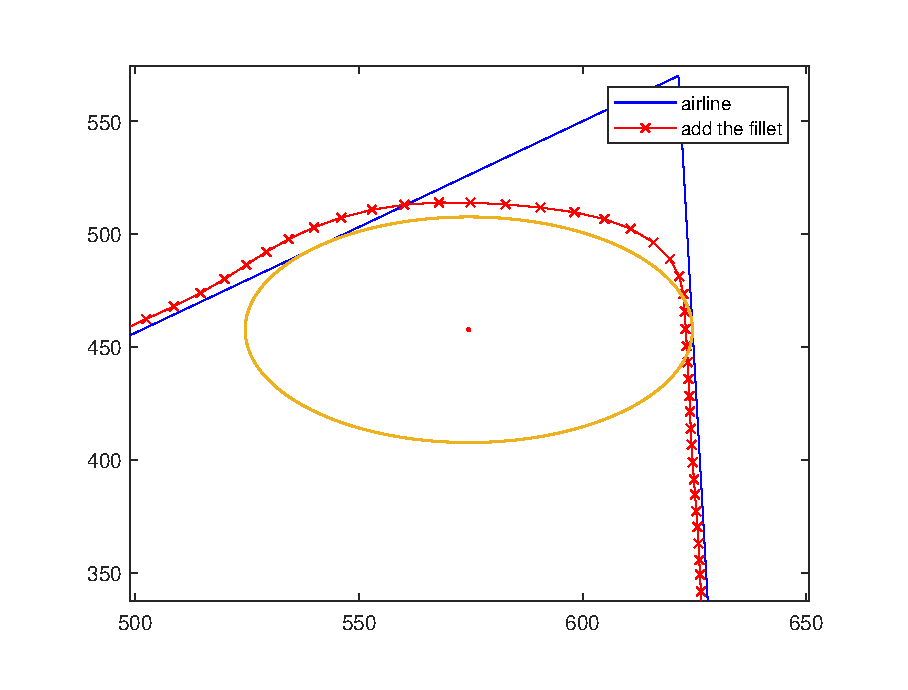
\includegraphics[width=0.8\textwidth]{pictures/eps/algorithm6_3.eps}
                \label{fig:algo6_3}
            \end{minipage}
        }
        \caption{algorithm6}
    \end{figure}
 
    对此提出了一个算法的改进. 根据图\ref{fig:algo6_1}, \ref{fig:algo6_2}, \ref{fig:algo6_3}显示, 超出航线的那一小部分还是由于惯性动量导致的, 所以在这里我们需要提前来进行航先切换, 从而留出一部分来减弱惯性动量, 让转弯轨迹更加的圆滑, 航线执行总的距离更小. 故对算法\ref{algo6:ref}进行了改进, 从而得到了算法\ref{algo6_opti:ref}.   
    \begin{figure}[htbp]
        \centering
        \subfigure[]{
            \begin{minipage}[t]{0.48\linewidth}
                \centering
                    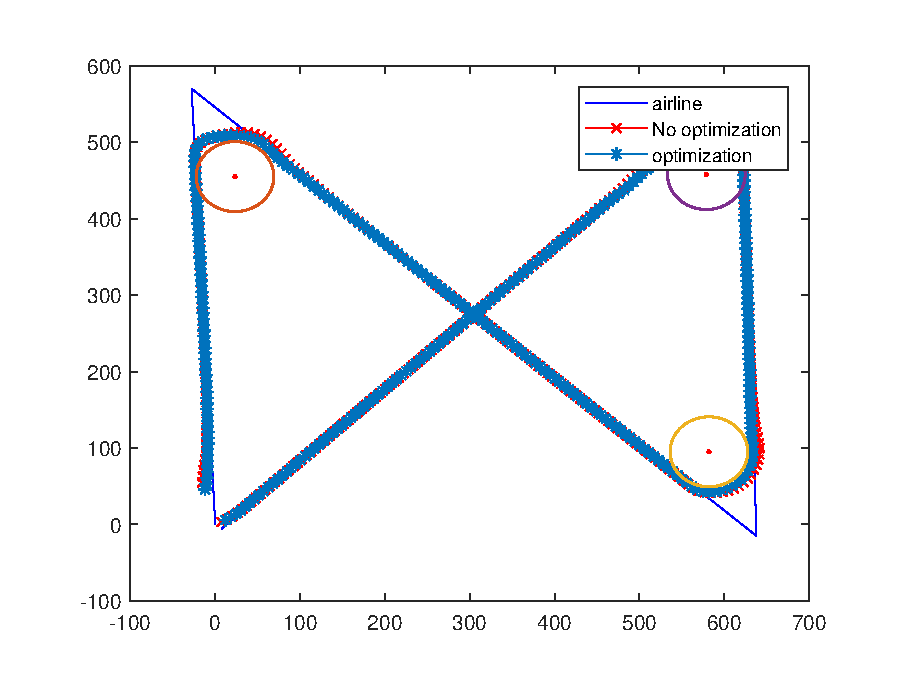
\includegraphics[width=0.7\textwidth]{pictures/eps/algorithm7.eps}
                \label{fig:algo7}
            \end{minipage}
        }
        \subfigure[]{
            \begin{minipage}[t]{0.48\linewidth}
                \centering
                    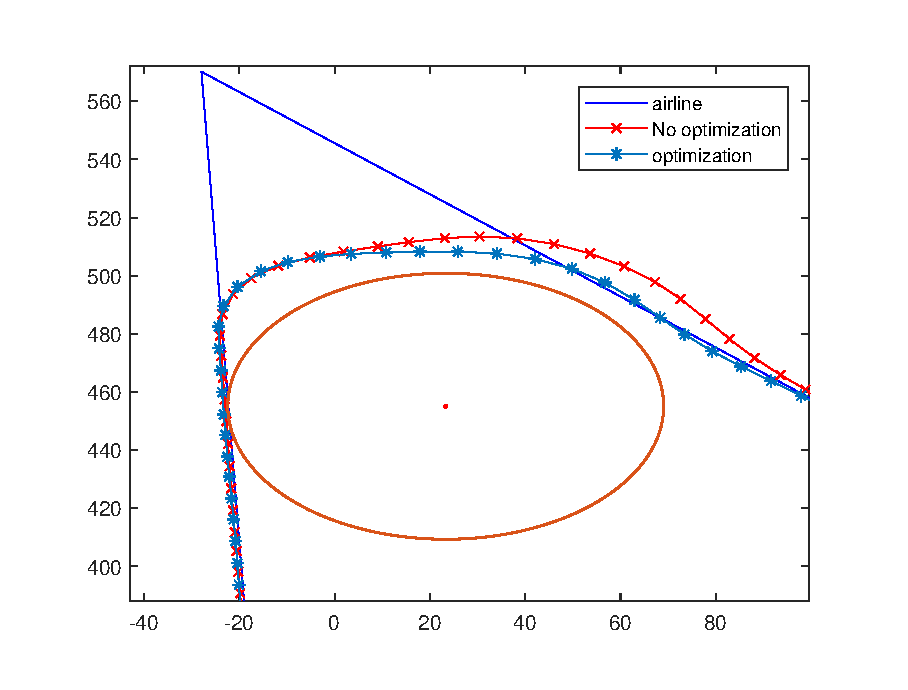
\includegraphics[width=0.7\textwidth]{pictures/eps/algorithm7_1.eps}
                \label{fig:algo7_1}
            \end{minipage}
        }
        \\
        \subfigure[]{
            \begin{minipage}[t]{0.48\linewidth}
                \centering
                    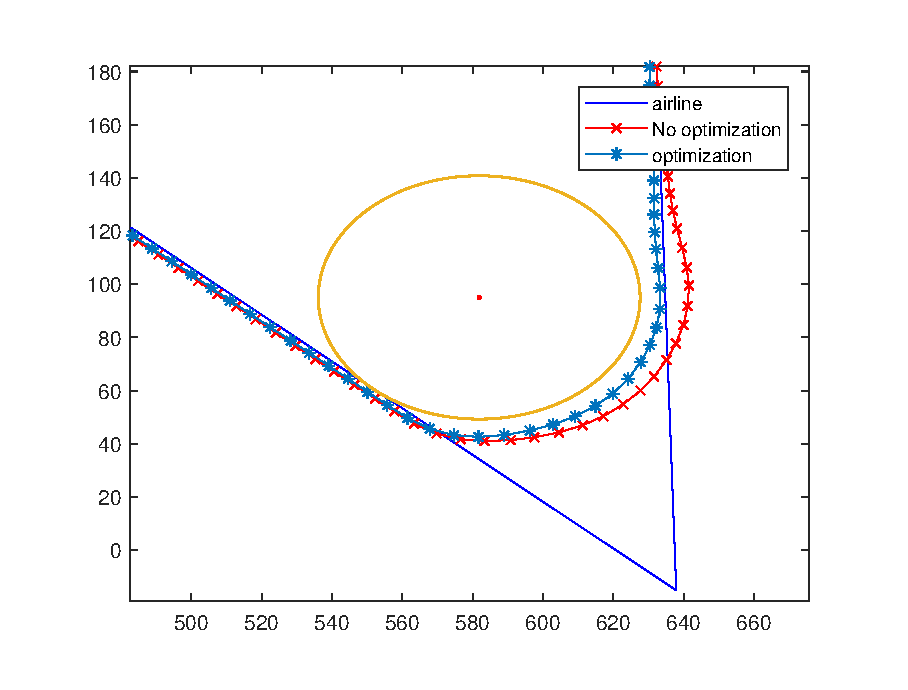
\includegraphics[width=0.7\textwidth]{pictures/eps/algorithm7_2.eps}
                \label{fig:algo7_2}
            \end{minipage}
        }
        \subfigure[]{
            \begin{minipage}[t]{0.48\linewidth}
                \centering
                    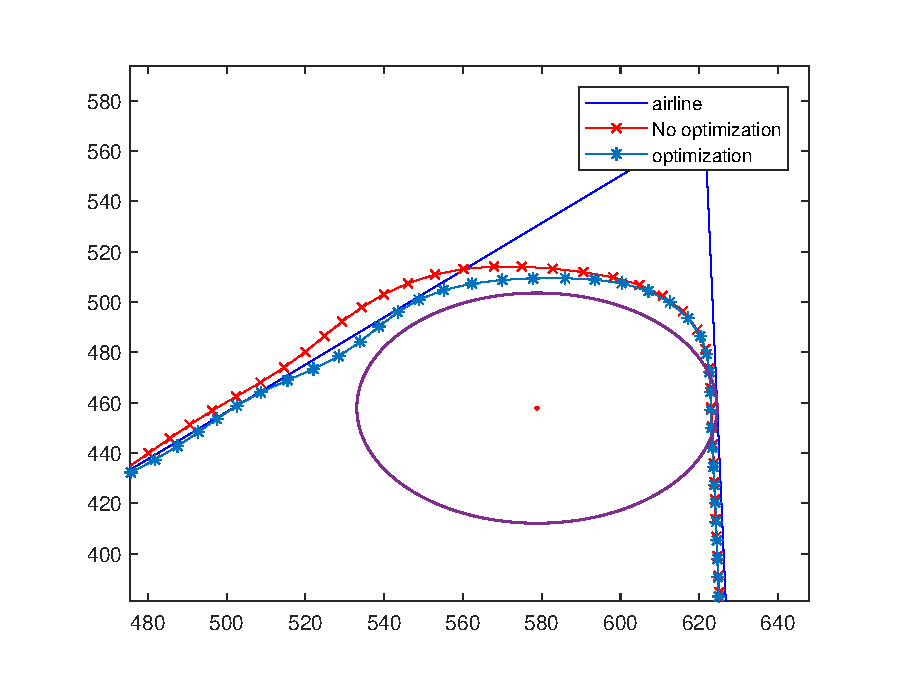
\includegraphics[width=0.7\textwidth]{pictures/eps/algorithm7_3.eps}
                \label{fig:algo7_3}
            \end{minipage}
        }
        \caption{algorithm6 comparing 1}
    \end{figure}
    
    \par 算法中, 在\ref{algo7_z1}行, 保存第一个半平面与航线$\overline{w_{i-1}w_{i}}$的交点$z$为$z_{1}$, 
    当进入第一个半平面的时候,state = 2,执行曲线控制逻辑,对应的圆心为第\ref{new_center}行所示的$c$, 其中半径进行了一定比例的缩放,已到达保留一定的距离来消耗无人机初始惯性动量的目的。第20行和22行,对应的R都进行了比例缩放,其中第20行是为fillet center设置半径,第22行是计算新的第二个半平面和下一条航线的新交点;第23行判断是否到达第二个半平面,若到达则切换航线,state重新设置为1,执行直线控制逻辑;反之继续执行当前航线。
    前后算法比对的效果图如图\ref{fig:algo7}所示。
    \begin{algorithm}[t] % 算法6 的优化
        \caption{Follow Waypoints with Fillet:(flag, r, q, c, $\rho$, $\lambda$)=followWppFillet($\textit{W}$, p, $R$)}
        \label{algo6_opti:ref}
        \begin{algorithmic}[1]
            \ENSURE Waypoints path $\textit{W}$ = $\left\{ w_{1}, \dots, w_{N} \right\}$, MAV position p=$(p_{n}, p_{e}, p_{d})^{T}$, fillet radius $R$
            \REQUIRE N $\geq$ 3
            \IF {New waypoints path $\textit{W}$ is received}
                \STATE Initialize waypoint index: $i$ $\gets$ 2, and state machine: state $\gets$ 1
            \ENDIF
            \STATE $q_{i-1}$ $\gets$ $\frac{w_{i}-w_{i-1}}{\lVert w_{i}-w_{i-1} \rVert}$
            \STATE $q_{i}$ $\gets$ $\frac{w_{i+1}-w_{i}}{\lVert w_{i+1}-w_{i} \rVert}$
            \STATE $\varrho$ $\gets$ $cos^{-1}(-q_{i-1}^{T}q_{i})$
            \IF {state = 1}
                \STATE flag $\gets$ 1
                \STATE $r$ $\gets$ $w_{i-1}$
                \STATE $q$ $\gets$ $q_{i-1}$
                \STATE $z$ $\gets$ $w_{i} - \frac{R}{tan(\frac{\varrho}{2})}q_{i-1}$
                \STATE $z_{1}$ $\gets$ $z$     \label{algo7_z1}   
                \IF {$p$ $\in$ $\textit{H}(z,q_{i-1})$}
                    \STATE state $\gets$ 2
                \ENDIF
            \ELSIF{state = 2}
                \STATE flag $\gets$ 2
                
                % 计算新的 center >>>>>>>>>>>>>>>>> 
                \STATE $c$ $\gets$ $w_{i} - \frac{R}{sin(\frac{\varrho}{2})}\frac{q_{i-1}-q_{i}}{\lVert q_{i-1}-q_{i} \rVert}$
                \STATE $c$ $\gets$ $z_{1} + \frac{c-z_{1}}{\lVert c-z_{1}\rVert}*0.915R$ %  \frac{R}{sin(\frac{\varrho}{2})}\frac{q_{i-1}-q_{i}}{\lVert \| q_{i-1}-q_{i} \rVert}$
                \label{new_center}
                \STATE $\rho$ $\gets$ $0.915R$
                % <<<<<<<<<<<<<<<<< 计算新的 center

                \STATE $\lambda$ $\gets$ $sign(q_{i-1,n}q_{i,e}-q_{i-1,e}q_{i,n})$
                \STATE $z_{2}$ $\gets$ $w_{i} + \frac{1}{tan(\frac{\varrho}{2})}*0.915R*q_{i}$
                \IF {$p$ $\in$ $\textit{H}(z,q_{i})$}
                    \STATE $i$ $\gets$ $\left(i+1\right)$ until $i$ = $N$ - 1
                    \STATE state $\gets$ 1
                \ENDIF
            \ENDIF
            \RETURN flag, $r$, $q$, $c$, $\rho$,$\lambda$.  % this command shows "Output"
        \end{algorithmic}
    \end{algorithm}
    \subsubsection{误差分析}
    \begin{center} 
        \begin{table}[H]
            \caption{误差分析表}
            \label{tab1}
            \begin{tabular}{c|c|c|c|c}
                \hline
                & 第一段(*150)& 第二段((*130))& 第三段(*120) &总和 \\
                \hline
                优化之前 &9.506485437269829& 13.459338133308067& 12.517388189403794 & 11.694433389122446 \\
                \hline
                优化之后 &9.307437579575690& 2.896129449605189& 7.097844734906930 & 6.560884583934650 \\
                \hline
                % \caption{误差分析表}
            \end{tabular} 
        \end{table}   
    \end{center}
    
    通过计算超出航线部分的点到航线的垂直距离,即偏离航线的误差,来判定算法是否优化。算法优化之前和优化之后误差分析如\ref{tab1}所示。
    最终计算得到的总的偏差由11.7减少到6.6,效果优化了78\%,足以可见算法\ref{algo6_opti:ref}较之前算法具有很好的效用性。
